\documentclass[supercite]{Experimental_Report}

\title{~~~~~~计算机视觉实验四~~~~~~}
\author{崔昊阳}
\school{计算机科学与技术学院}
\classnum{CS2104}
\stunum{U202115415}
\instructor{刘康}
\date{2023年12月20日}

\usepackage{algorithm, multirow}
\usepackage{algpseudocode}
\usepackage{amsmath}
\usepackage{amsthm}
\usepackage{framed}
\usepackage{mathtools}
\usepackage{subcaption}
\usepackage{xltxtra}
\usepackage{bm}
\usepackage{tikz}
\usepackage{tikzscale}
\usepackage{pgfplots}
\usepackage{listings}
\lstset{
    backgroundcolor = \color{white},    % 背景色
    basicstyle = \small\ttfamily,           % 基本样式 + 小号字体
    rulesepcolor= \color{white},             % 代码块边框颜色
    breaklines = true,                  % 代码过长则换行
    numbers = left,                     % 行号在左侧显示
    numberstyle = \small,               % 行号字体
    keywordstyle = \color{blue}\bfseries,      % 关键字颜色
	identifierstyle=\color{purple}, 		% 标识符颜色
    commentstyle =\color{green},        % 注释颜色
    stringstyle = \color{green},          % 字符串颜色
    frame = None,                  % 用(带影子效果)方框框住代码块
    showspaces = false,                 % 不显示空格
    columns = flexible,                    % 字间距固定
}

\pgfplotsset{compat=1.16}

\newcommand{\cfig}[3]{
  \begin{figure}[H]
    \centering
    \includegraphics[width=#2\textwidth]{images/#1.tikz}
    \caption{#3}
    \label{fig:#1}
  \end{figure}
}

\newcommand{\sfig}[3]{
  \begin{subfigure}[b]{#2\textwidth}
    \includegraphics[width=\textwidth]{images/#1.tikz}
    \caption{#3}
    \label{fig:#1}
  \end{subfigure}
}

\newcommand{\xfig}[3]{
  \begin{figure}[H]
    \centering
    #3
    \caption{#2}
    \label{fig:#1}
  \end{figure}
}

\newcommand{\rfig}[1]{\autoref{fig:#1}}
\newcommand{\ralg}[1]{\autoref{alg:#1}}
\newcommand{\rthm}[1]{\autoref{thm:#1}}
\newcommand{\rlem}[1]{\autoref{lem:#1}}
\newcommand{\reqn}[1]{\autoref{eqn:#1}}
\newcommand{\rtbl}[1]{\autoref{tbl:#1}}

\algnewcommand\Null{\textsc{null }}
\algnewcommand\algorithmicinput{\textbf{Input:}}
\algnewcommand\Input{\item[\algorithmicinput]}
\algnewcommand\algorithmicoutput{\textbf{Output:}}
\algnewcommand\Output{\item[\algorithmicoutput]}
\algnewcommand\algorithmicbreak{\textbf{break}}
\algnewcommand\Break{\algorithmicbreak}
\algnewcommand\algorithmiccontinue{\textbf{continue}}
\algnewcommand\Continue{\algorithmiccontinue}
\algnewcommand{\LeftCom}[1]{\State $\triangleright$ #1}

\newtheorem{thm}{定理}[section]
\newtheorem{lem}{引理}[section]

\colorlet{shadecolor}{black!15}

\theoremstyle{definition}
\newtheorem{alg}{算法}[section]

\def\thmautorefname~#1\null{定理~#1~\null}
\def\lemautorefname~#1\null{引理~#1~\null}
\def\algautorefname~#1\null{算法~#1~\null}

\begin{document}

\maketitle

\clearpage

\pagenumbering{Roman}

\tableofcontents[level=2]

\clearpage

\pagenumbering{arabic}

\section{实验要求}
任务要求:针对已训练好的卷积神经网络,给定一张输入图片,生成该图片对于特定类别的可解释性分析结果。

实验将提供基于 PyTorch 和 TensorFlow 的两个不同版本的二分类模型,该模型可用于猫和狗的分类(class 0 为猫,class 1 为狗)。注:PyTorch 使用的网络架构是 AlexNet,TensorFlow 使用的是 VGG16,两者略有不同,请任选一个模型进行实验。

实验将同时提供三张输入图片,对于每张图片,分别针对猫和狗的类别,进行GradCAM和LayerCAM的可解释性分析。

注意事项:
\begin{enumerate}
	\item 深度学习框架可选 PyTorch 和 TensorFlow。
	\item 实验报告需包含每张输入图片在最后一层卷积层输出的的可视化结果(对输出特征图的每一个通道进行可视化),每张图片分别针对猫和狗两个类别的可解释性分析结果(Grad-CAM 及 LayerCAM),以及对应的实验分析。
	\item 将代码和实验报告打包成 ZIP 压缩包,以“姓名-学号-实验报告\#”命名,比如“张三-2020XXX-实验报告四.zip”,提交到学习通。
	\item 截止时间为 1 月 10 号下午 2:00。
\end{enumerate}

\section{数据集读取}
本次实验中的数据处理部分相对简单,仅需要读取 3 张用于测试的图片。
我们编写了一个支持迭代的数据集类,用于将 3 张用于测试的图片转换成可输入模型的形式。在实例化此类时,我们传入
测试集的地址。在每次迭代时,实例会读入对应的图像并将其转换成 Tensor 格式返回。具体代码如下。
\begin{lstlisting}
class PicDataset(Dataset):
"""
猫狗分类的 Dataset
:params data_path: 数据集路径
"""

def __init__(self, data_path: str):
    super().__init__()
    self.data_path = data_path
    self.data_info = os.listdir(self.data_path)
    self.transform = transforms.Compose([transforms.ToTensor()])

def __getitem__(self, index):
    img_path = os.path.join(self.data_path, self.data_info[index])
    img = self.transform(Image.open(img_path))
    return img

def __len__(self):
    return len(self.data_info)
\end{lstlisting}

\section{可解释性分析算法}
可解释性是指以可理解的方式向人类提供解释的能力。而深度学习模型的可解释性是指解释和理解模型如何做出预测和决策。
可解释性分析算法可以揭示模型的行为,并提供对模型预测的解释。
深度学习模型的可解释性具有重要意义,它可以帮助我们提高模型的可靠性,发现模型的缺点以及满足一些法律、伦理上的要求。

在本章中,我们将介绍本次实验使用的两种可解释性分析算法: GradCAM 和 LayerCAM。
我们首先介绍 CAM 可视化,接着介绍 GradCAM 和 LayerCAM。
\subsection{CAM}
CAM 算法(类激活映射算法)是由 Bolei Zhou 等人于 2016 年提出的,用于可视化卷积神经网络在图像分类任务中的关注区域的可解释性分析算法。
CAM 算法的大致流程如图\ref{CAM}所示,其具体过程如下。
\begin{figure}[H]
	\begin{center}
		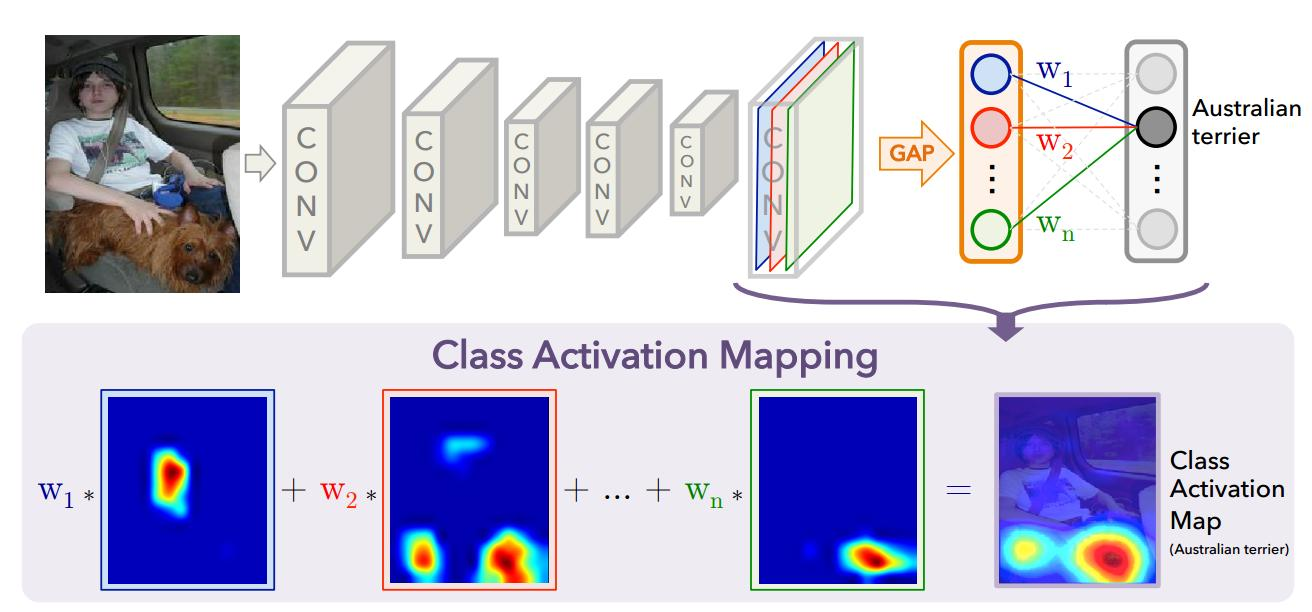
\includegraphics[scale=0.25]{../images/CAM算法结构图.png}
		\caption{CAM 算法结构图}
		\label{CAM}
	\end{center}
\end{figure}

首先,CAM 算法将卷积神经网络的最后一层的输出进行全局平均池化(GAP)操作,获取在最后一个卷积层的各单元特征图的空间平均值。
\begin{equation}
  P_k=\frac{1}{N^2}\sum_{i=1}^{N}\sum_{j=1}^{N}A_k(i, j)
\end{equation}

其中,$A_k(i, j)$ 是最后一个卷积层上的第 $k$ 个通道的特征图,$P_k$ 是第 $k$ 个通道的全局平均池化结果,$N$ 是图像的分辨率。

接着,我们对每个通道的全局平均池化结果进行加权平均,得到每个分类的 logit。
\begin{equation}
  L_c=\sum_{k=1}^{K}w_k^cP_k
\end{equation}

其中,$w_k^c$ 是分类 $c$ 在第 $k$ 个通道上的权重,$P_k$ 是第 $k$ 个通道上的全局平均池化值,$K$ 是输入图像的通道总数。

然后使用 \texttt{softmax} 函数得到每个类别的概率分布并选择概率最大的类别作为目标类。训练完成后,我们将得到一组合适的权重 $w$。

最后,将训练好的权重与最后一层卷积的图像进行加权求和后经过 ReLU 激活函数,并上采样到和原始图像一样的大小,即可得到 CAM 热力图。
\begin{eqnarray}
  CAM_c(i, j)=max\{\sum_{k=1}^{K}w_k^cA_k(i, j), 0\}
\end{eqnarray}

其中,$w_k^c$ 是分类 $c$ 在第 $k$ 个通道上的权重,$A_k(i, j)$是最后一个卷积层上的第 $k$ 个通道的特征图,$K$ 是输入图像的通道总数。

CAM 算法可以提供直观的模型预测解释。但是,CAM 算法也存在着诸多缺陷。
首先,CAM 只能分析最后一层卷积层输出,无法分析中间层。
其次,CAM 只适用于图像分类任务。上述两个缺点限制了 CAM 的应用范围。
最后,CAM 要求模型必须有 GAP 层,否则需要修改模型并重新训练,这降低了 CAM 算法的应用方便性。
因此,人们提出了基于 CAM 算法的许多改进算法,如 GradCAM,LayerCAM。

\subsection{GradCAM}
GradCAM 是对 CAM 算法的改进,由 Ramprasaath R.Selvaraju 等人于 2017 年提出。
和 CAM 不同,GradCAM 会利用梯度信息来确定哪些区域对于特定类别的预测是最重要的。
GradCAM 算法的大致流程如图\ref{GradCAM}所示,其具体过程如下。
\begin{figure}[H]
	\begin{center}
		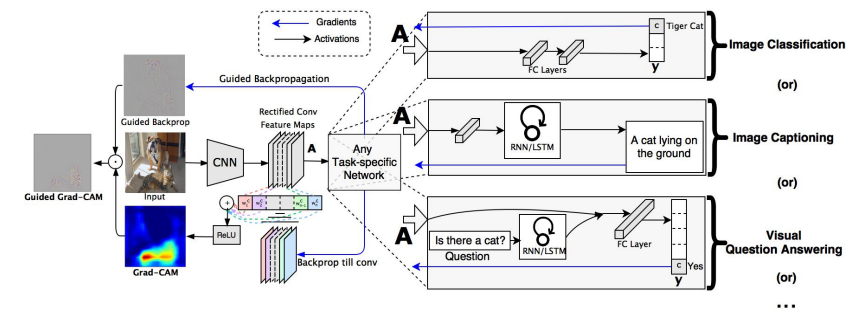
\includegraphics[scale=0.6]{../images/GradCAM算法结构图.png}
		\caption{GradCAM 算法结构图}
		\label{GradCAM}
	\end{center}
\end{figure}

首先,GradCAM 计算目标类别在最后一层卷积层的梯度。
\begin{equation}
g_k^c(i, j) = \frac{\partial l^c}{\partial A_k(i, j)}
\end{equation}

其中,$g_k^c$ 是类别 $c$ 在第 $k$ 个通道上的梯度矩阵,$l^c$ 是类别 $c$ 的 logits,$A_k$ 是目标层的第 $k$ 通道的特征图。

接着,我们对梯度进行全局平均池化操作,获取各通道的权重。
\begin{equation}
w_k^c=\frac{1}{N^2}\sum_{i=1}^{N}\sum_{j=1}^{N}g_k^c(i, j)
\end{equation}

其中,$w_k^c$ 是各通道的权重,$g_k^c$ 是类别 $c$ 在第 $k$ 个通道上的梯度矩阵,$N$ 是图像的分辨率。

最后,我们将各通道的特征图加权求和并经 ReLU 去除负值,得到最终的类激活映射。
\begin{equation}
GCAM_c(i, j)=max\{\sum_{i=1}^{K}w_k^cA_k(i, j), 0\}
\end{equation}

其中,$w_k^c$ 是分类 $c$ 在第 $k$ 个通道上的权重,$A_k$ 是目标层的第 $k$ 通道的特征图,$K$ 是输入图像的通道总数。

GradCAM 不要求模型必须有GAP层,不修改网络结构,不需要重新训练。同时,它还可以应用于 CNN 的任意卷积层。
但是,GradCAM 同样存在着一些缺陷。
首先,GradCAM 的深层生成的粗粒度热力图和浅层生成的细粒度热力图都不够精确。
其次,对于层数较浅的卷积层,GradCAM 的分析效果较差。
因此,人们提出了 LayerCAM,对 GradCAM 进行了改进。

\subsection{LayerCAM}
LayerCAM 是对 GradCAM 的改进,由 PengTao Jiang 等人于 2019 年提出。
相比于 GradCAM,LayerCAM 对特征图的梯度进行元素级的乘法而不是进行全局平均池化操作。这使得 LayerCAM 可以生成更精细的类别激活图。
LayerCAM 算法的具体过程如下。

首先,和 GradCAM 相同,LayerCAM 计算目标类别在最后一层卷积层的梯度。
\begin{equation}
g_k^c(i, j) = \frac{\partial l^c}{\partial A_k(i, j)}
\end{equation}

其中,$g_k^c$ 是类别 $c$ 在第 $k$ 个通道上的梯度矩阵,$l^c$ 是类别 $c$ 的 logits,$A_k$ 是目标层的第 $k$ 通道的特征图。

接着,每个通道上的梯度矩阵经 ReLU 函数得到每个通道上的各元素权重。
\begin{equation}
w_k^c(i,j)=max\{g_k^c(i,j),0\}
\end{equation}

其中,$w_k^c$ 是分类 $c$ 在第 $k$ 个通道上的权重矩阵,$g_k^c$ 是类别 $c$ 在第 $k$ 个通道上的梯度矩阵。

最后,我们将各通道的特征图和其对应的权重矩阵逐元素相乘,再将各通道的相同位置的元素相加并经 ReLU 去除负值,得到最终的类激活映射。
\begin{equation}
LCAM_c(i,j)=max\{\sum_{i=1}^{K}w_k^c(i,j)\cdot A_k(i,j),0\}
\end{equation}

其中,$w_k^c$ 是分类 $c$ 在第 $k$ 个通道上的权重矩阵,$A_k$ 是目标层的第 $k$ 通道的特征图,$K$ 是输入图像的通道总数。

\section{实验结果}
\subsection{实验环境}
本实验在本地笔记本电脑上进行,配置如表\ref{服务器配置}所示。
同时,为了使结果可复现,我们将随机数种子固定为 1024。我们还使用了 GPU 加速训练。
\begin{table}[H]
	\centering
	\caption{实验环境表}
	  \begin{tabular}{c|c|c}
		\toprule
	  \multirow{3}[0]{*}{硬件} & CPU   & 11th Gen Intel(R) Core(TM) i7-11800H @ 2.30GHz \\
			& 内存大小    & 16G \\
			& GPU   & NVIDIA GeForce RTX 3060 Laptop GPU \\\hline
	  \multirow{3}[0]{*}{软件} & 操作系统  & Windows 11 \\
			& 深度学习框架 & PyTorch 1.13.0 \\
			& IDE   & Vscode \\\bottomrule
	  \end{tabular}
	\label{服务器配置}
\end{table}

\subsection{结果}
我们分别复现了 GradCAM 和 LayerCAM。我们的基础模型采用了 PyTorch 框架下的 AlexNet 猫狗分类的模型。
我们使用了 3 张图片:一张为猫、一张为狗。一张同时存在猫和狗,对两种 CAM 算法进行了测试。
在实验中我们分析的特征图是最后一层卷积层经 ReLU 和 MaxPool2d 之后的特征图。测试的结果如下。

首先我们对三张图片的输出特征图各通道进行可视化。
如图\ref{特征图1}、\ref{特征图2}和\ref{特征图3}所示。

当我们使用 GradCAM 可解释性分析算法时,
最终的 CAM 热力图如图 \ref{GradCAM热力图}所示。

当我们使用 LayerCAM 可解释性分析算法时,
最终的 CAM 热力图如图 \ref{LayerCAM热力图}所示。
\begin{figure}[H]
	\begin{center}
		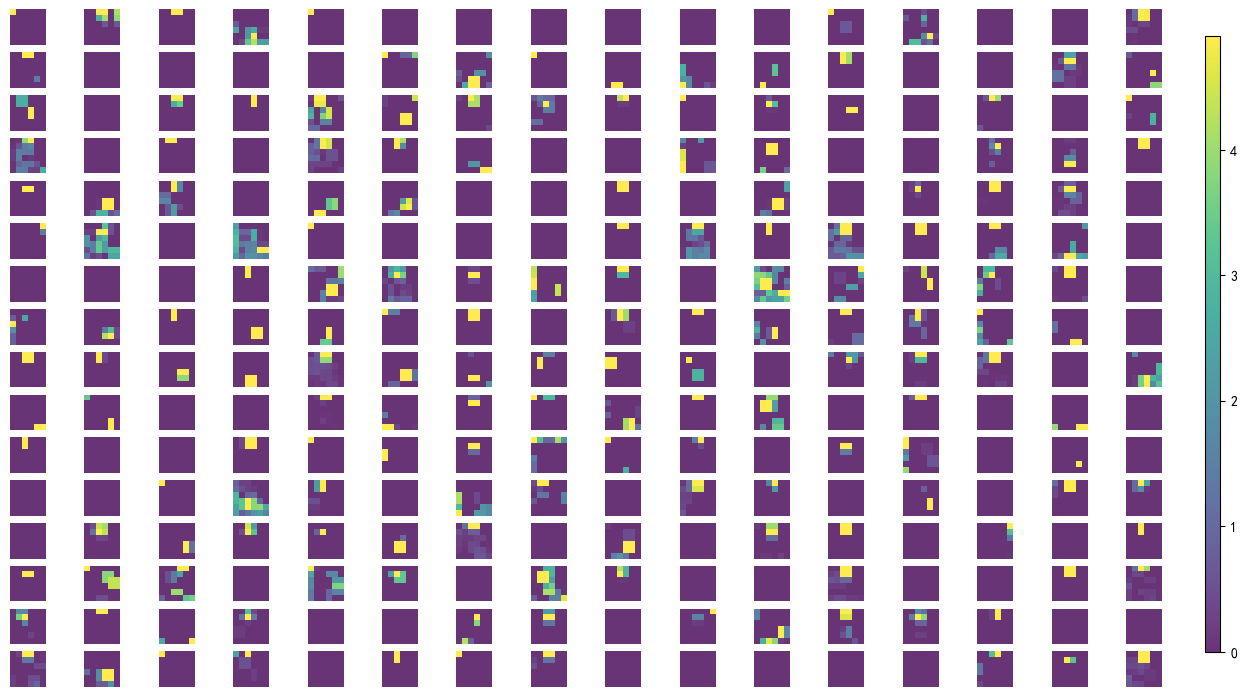
\includegraphics[scale=0.35]{../images/feature-map0.png}
		\caption{both 特征图}
		\label{特征图1}
	\end{center}
\end{figure}
\begin{figure}[H]
	\begin{center}
		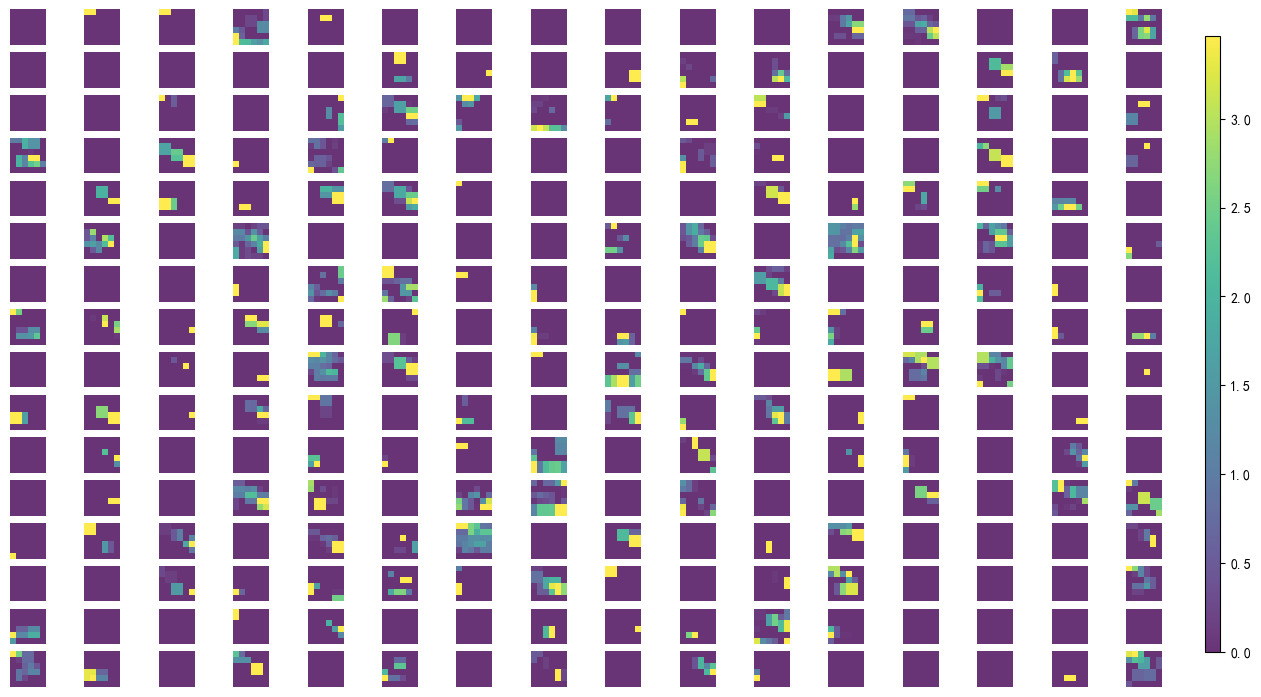
\includegraphics[scale=0.35]{../images/feature-map1.png}
		\caption{cat 特征图}
		\label{特征图2}
	\end{center}
\end{figure}
\begin{figure}[H]
	\begin{center}
		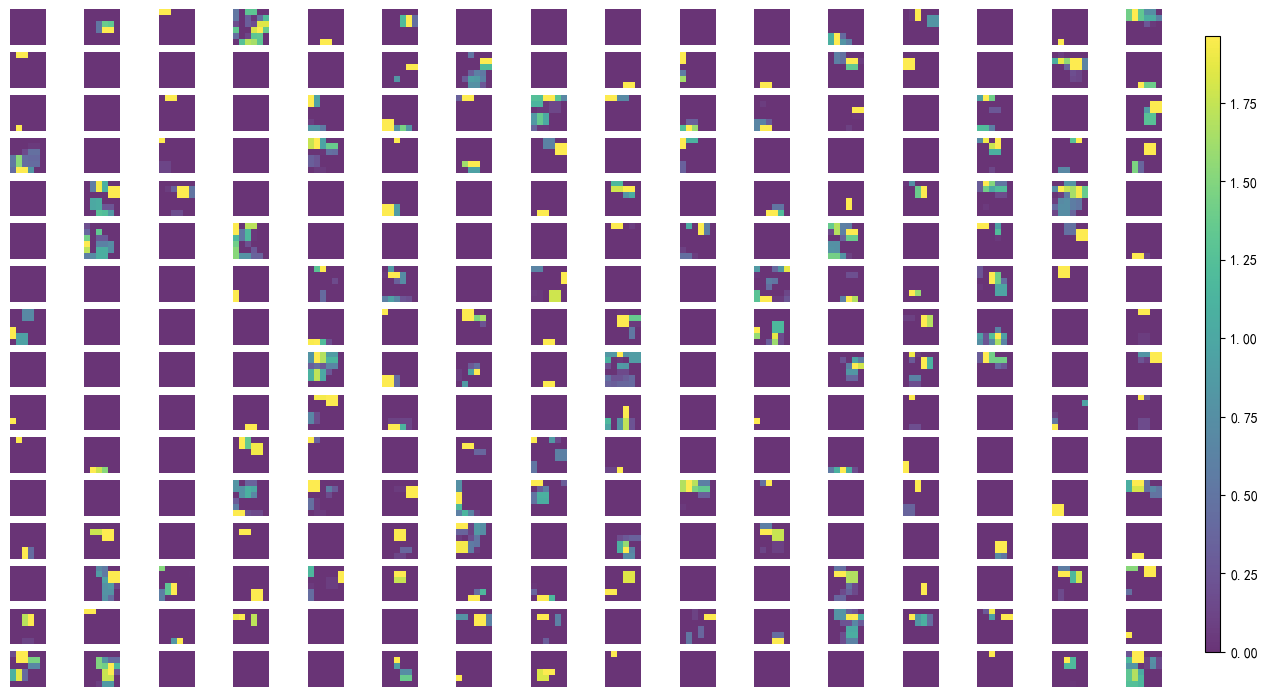
\includegraphics[scale=0.35]{../images/feature-map2.png}
		\caption{dog 特征图}
		\label{特征图3}
	\end{center}
\end{figure}
\begin{figure}[H]
	\begin{center}
		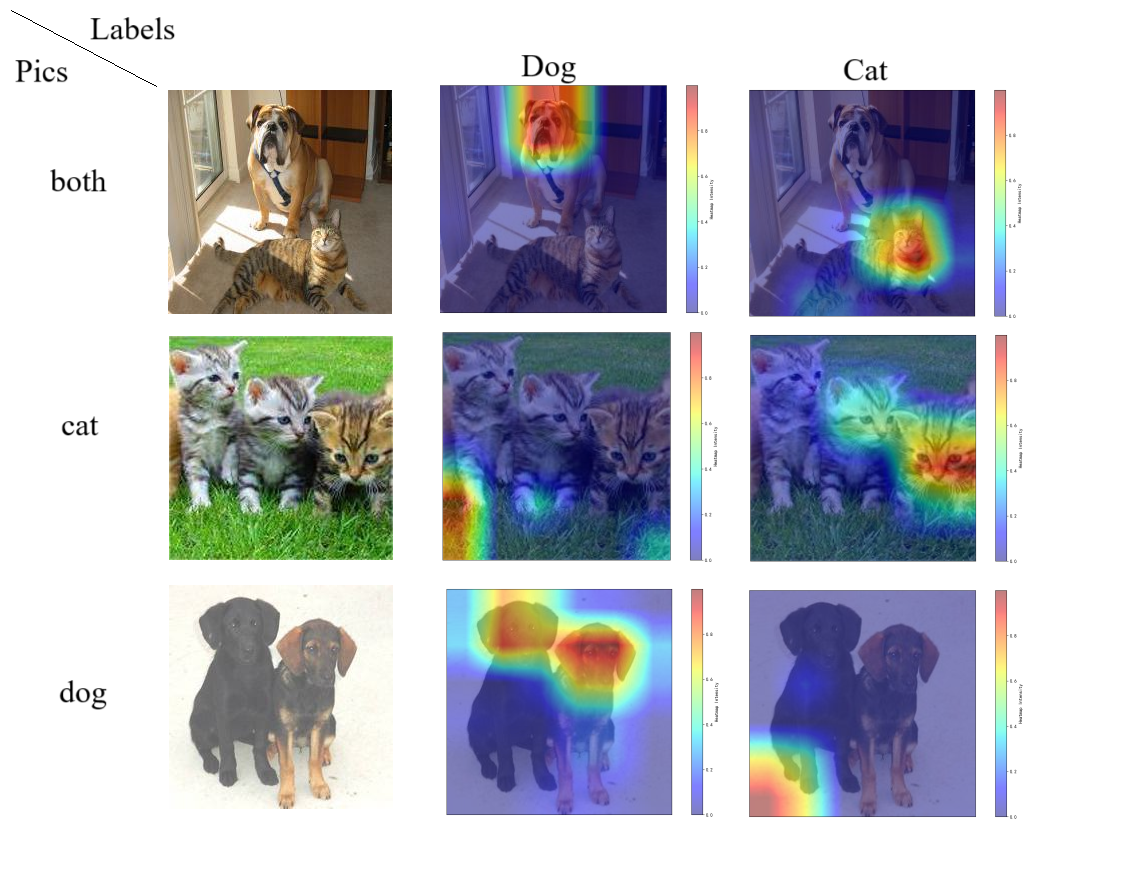
\includegraphics[scale=0.55]{../images/GradCAM热力图.png}
		\caption{GradCAM 热力图}
		\label{GradCAM热力图}
	\end{center}
\end{figure}
\begin{figure}[H]
	\begin{center}
		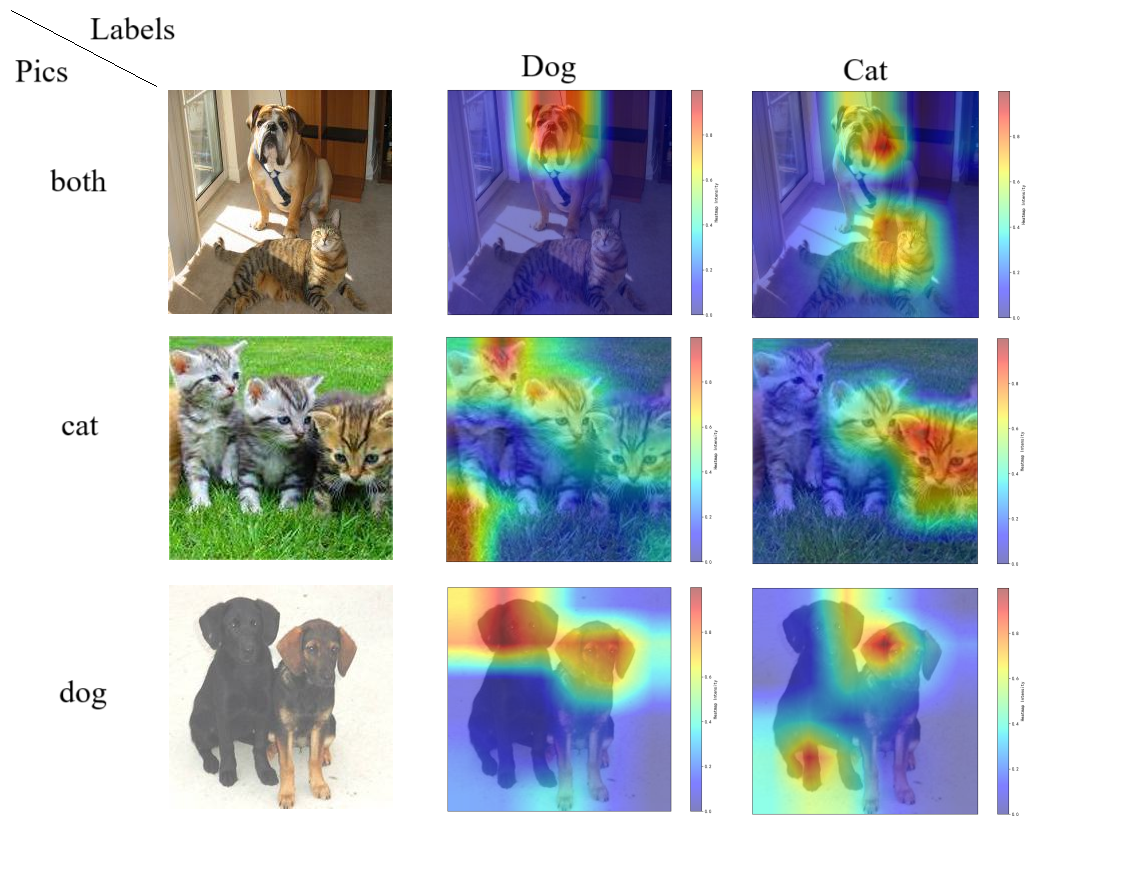
\includegraphics[scale=0.55]{../images/LayerCAM热力图.png}
		\caption{LayerCAM 热力图}
		\label{LayerCAM热力图}
	\end{center}
\end{figure}
\section{总结与讨论}
在这一章,我们主要对 GradCAM 和 LayerCAM 两种不同的可解释性分析算法的实验结果进行讨论。

最后一层卷积层的特征图表示输入图像的深层特征。
我们观察特征图的可视化结果\ref{特征图1}、\ref{特征图2}和\ref{特征图3},发现它们并不能为人类所直观地理解。
所以,我们只能通过 CAM 等可解释性分析算法来理解这些特征图的含义。

两种不同的可解释性分析算法在正确标签上的实验结果对比图如图\ref{对比图}所示。
\begin{figure}[H]
	\begin{center}
		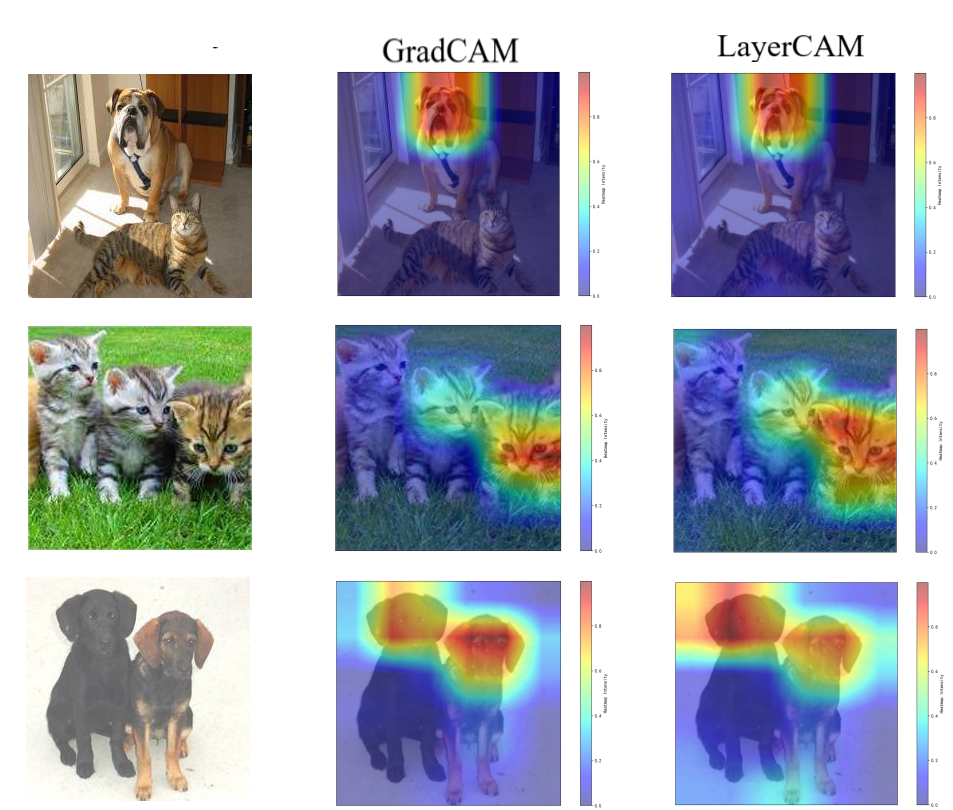
\includegraphics[scale=0.7]{../images/all.png}
		\caption{实验结果对比图}
		\label{对比图}
	\end{center}
\end{figure}

从图\ref{对比图}中我们可以看出两种方法的结果差异不大,它们都成功显示了模型在进行分类时关注的图片区域。

对于 both 图片,我们发现模型在分类为狗时关注狗的面部,而分类为猫时关注猫的面部。
模型最终分类为狗的原因可能是狗的面部占据的面积大于猫的面部占据的面积,而模型主要通过面部的特征来进行分类。

对于 cat 图片,我们发现模型最关注从左向右第三只小猫的面部,也关注了中间的小猫面部,而几乎未关注从左向右第一只小猫。
所以模型分类为猫。模型对三只小猫的关注差异可能和它们面部的角度有关。小猫的正向面部相较于侧向面部,含有更多猫的特征,所以更容易被模型所关注。
由于这张图片中没有狗,所以分类为狗时的热力图没有意义。

对于 dog 图片,我们发现模型关注了图片中两只狗的面部。所以模型分类为狗。由于两只狗的面部全部是正向,含有的特征信息数量差异不大,
所以模型同时关注了它们。由于这张图片中没有猫,所以分类为猫时的热力图没有意义。

\section{实验代码简述}
在本章中,我们简要介绍实验代码的构成。更具体的介绍请见 ReadMe.md 文件。

工作目录中存在 5 个文件和 2 个目录。整个工作目录的结构如下。
\begin{figure}[H]
	\begin{center}
		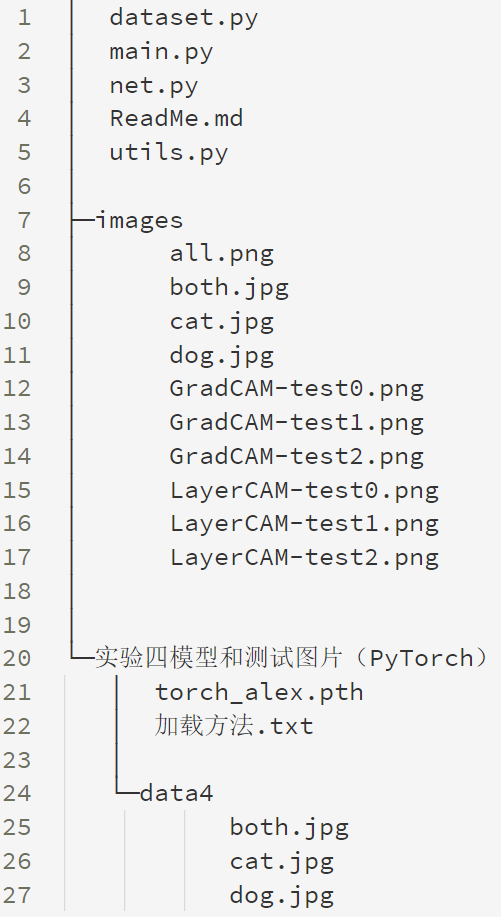
\includegraphics[scale=0.5]{../images/tree.png}
		\caption{工作目录的结构}
	\end{center}
\end{figure}

其中,dataset.py 中含有数据预处理的相关函数。net.py 含有可解释性分析算法的定义和实现。
ReadMe.md 中介绍了如何对模型进行训练和测试。main.py 是实现可解释性计算的主程序。
utils.py 中含有一些工具函数。各函数和类的源代码均含有详细的注释,方便使用者了解其完成的工作。
images 目录存放所有绘制的图像。

\end{document}